\documentclass{report}
\usepackage{graphicx} % Required for inserting images
\usepackage[italian]{babel}
\usepackage{hyphenat}
\hyphenation{}
\usepackage{hyperref}
\hypersetup{
    colorlinks,
    citecolor=black,
    filecolor=black,
    linkcolor=black,
    urlcolor=black
}
\usepackage{listings}
\renewcommand{\lstlistingname}{} % This removes the word "Listing"

\usepackage{xcolor}

%New colors defined below
\definecolor{codegreen}{rgb}{0,0.6,0}
\definecolor{codegray}{rgb}{0.5,0.5,0.5}
\definecolor{codepurple}{rgb}{0.58,0,0.82}
\definecolor{backcolour}{rgb}{0.95,0.95,0.92}

%Code listing style named "mystyle"
\lstdefinestyle{mystyle}{
  backgroundcolor=\color{backcolour}, commentstyle=\color{codegreen},
  keywordstyle=\color{magenta},
  numberstyle=\tiny\color{codegray},
  stringstyle=\color{codepurple},
  basicstyle=\ttfamily\footnotesize,
  breakatwhitespace=false,         
  breaklines=true,                 
  captionpos=b,                    
  keepspaces=true,                 
  numbers=left,                    
  numbersep=5pt,                  
  showspaces=false,                
  showstringspaces=false,
  showtabs=false,                  
  tabsize=2
}

%"mystyle" code listing set
\lstset{style=mystyle}

\title{Distance Vector Routing}
\author{Andrea Baldazzi : 0001071149}
\date{\today}

\begin{document}

\maketitle

\tableofcontents

\chapter{Introduzione}
L'elaborato simula il funzionamento del protocollo \emph{Distance Vector Routing}, implementato con un semplice programma Python. 

\chapter{Funzionamento}
Ogni router virtuale tiene traccia delle rotte migliori associando ad ogni nodo (router) da esso raggiungibile un costo e il primo nodo da cui passare per raggiungerlo. La simulazione prevede che i router scambino con i vicini il proprio Distance Vector e cerchino di migliorare il proprio in seguito alla ricezione degli altri Distance Vector.
\\\\Sono proposte due soluzioni, una semplice e una con meccanismi \emph{Split Horizon} e \emph{Triggered Update}.

\section{Soluzione semplice}
In questa implementazione viene proposto il meccanismo di \emph{Distance Vector Routing} così com'è senza meccanismi per facilitare la convergenza. Appropriata documentazione è presente nel codice Python sia per le classi che per i metodi.
\subsubsection{Creazione Router}
Nel programma un router è gestito come un oggetto con diverse funzionalità. Al momento della creazione viene creata una tabella di routing vuota, dove l'unica rotta è quella verso se stesso.
\begin{lstlisting}[language=Python, caption=Creazione router]
class Router:

    def __init__(self, name: str)
\end{lstlisting}
\subsubsection{Aggiunta router vicino}
Il router accetta l'aggiunta di un router vicino che viene subito aggiunto alla propria tabella di routing.
\begin{lstlisting}[language=Python, caption=Aggiunta router vicino]
def add_neighbour(self, neighbour: str, distance: int)
\end{lstlisting}
\subsubsection{Aggiornamento tabella}
Il router accetta un Distance Vector proveniente da un vicino e lo utilizza per aggiornare la propria tabella di routing. In particolare, vengono aggiunte le destinazioni non conosciute e aggiornate quelle già presenti nel caso venga fornita una rotta con minore distanza. Viene restituito True nel caso la tabella è stata modificata, False altrimenti.
\begin{lstlisting}[language=Python, caption=Aggiornamento tabella]
def update_table(self, neighbour: str, neighbour_table: dict[str, tuple[int, str]])
\end{lstlisting}
\subsubsection{Creazione rete}
Nel programma fornito la rete è implementata con un oggetto  con diverse funzionalità. Al momento della creazione è priva di router e di collegamenti.
\begin{lstlisting}[language=Python, caption=Creazione rete]
class Network:

    def __init__(self)
\end{lstlisting}
\subsubsection{Aggiunta collegamento tra router}
La rete permette di creare un nuovo collegamento tra due router. Nel caso essi non siano già presenti nella rete, vengono creati.
\begin{lstlisting}[language=Python, caption=Aggiunta colegamento tra router]
def add_edge(self, router1: str, router2: str, distance: int)
\end{lstlisting}
\subsubsection{Scambio dei distance vector}
La rete permette di far scambiare tra i router vicini i propri Distance Vector. Il processo viene ripetuto un numero di volte pari al numero di nodi nel caso il valore \verb|steps| non venga fornito.
\begin{lstlisting}[language=Python, caption=Scambio dei Distance Vector]
def update_tables(self, steps=None)
\end{lstlisting}

\section{Soluzione avanzata}
In questa implementazione viene modificato il programma semplice sopra descritto aggiungendo due meccanismi della rete per facilitare la convergenza della rete:
\begin{description}
  \item[Split Horizon:] Sfruttando la versione con Poisonous Reverse, se A per raggiungere C deve passare da B, dice a B che la sua distanza da C è infinita.
  \item[Triggered Update:] Ogni volta che un router aggiorna il suo Distance Vector lo invia a tutti i suoi vicini.
\end{description}
\subsubsection{Invio di un Distance Vector}
Con questo metodo un solo Distance Vector è inviato ai vicini, ovvero quello di \verb|router|. Il metodo tiene traccia di quali vicini hanno modificato la tabella, richiamandosi ricorsivamente su di essi per implementare \emph{Triggered Update}. Inoltre, ogni Distance Vector inviato è "avvelenato" per implementare \emph{Split Horizon}.
\begin{lstlisting}[language=Python, caption=Invio di un Distance Vector]
def send_table(self, router: str)
\end{lstlisting}
\subsubsection{Invio di tutti i Distance Vector}
Richiama \verb|send_table()| su tutti i nodi della rete un numero \verb|steps| di volte, pari al numero di router nella rete se non fornito.
\begin{lstlisting}[language=Python, caption=Invio di tutti i Distance Vector]
def update_tables(self, steps=None)
\end{lstlisting}

\chapter{Utilizzo}
\section{Avvio applicazione}
Per avviare l'applicazione è sufficiente, previa installazione di un interprete Python sulla propria macchina, avviare uno dei due script \verb|DV-routing-simulation.py| o \verb|DV+SH+TU-routing-simulation.py|. I due script sono stati testati con Python 3.11.8.
\section{Esempio dimostrativo}
Nei due script è precaricato un esempio di utilizzo, identico in entrambi. La rete è configurata nel seguente modo:
\begin{lstlisting}[language=Python]
net = Network()
net.add_edge("A", "B", 7)
net.add_edge("B", "C", 5)
net.add_edge("C", "D", 20)
net.add_edge("A", "D", 2)
\end{lstlisting}
Ne consegue che la struttura risultante sia la seguente:
\begin{figure}
{
    \centering
    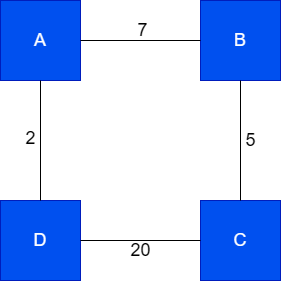
\includegraphics[width=0.3\linewidth]{DV-routing-example.png}
    \caption{Schema della rete di esempio}
    \label{fig:enter-label}
    }
\end{figure}
\\\\Forziamo ora lo scambio dei Distance Vector:
\begin{lstlisting}[language=Python]
net.update_tables()
net.print_tables()
\end{lstlisting}
L'output in console è il seguente:
\begin{lstlisting}[numbers=none]
Routing table for node A:
  Destination: A, Distance: 0, Next Hop: A
  Destination: B, Distance: 7, Next Hop: B
  Destination: D, Distance: 2, Next Hop: D
  Destination: C, Distance: 12, Next Hop: B
Routing table for node B:
  Destination: B, Distance: 0, Next Hop: B
  Destination: A, Distance: 7, Next Hop: A
  Destination: C, Distance: 5, Next Hop: C
  Destination: D, Distance: 9, Next Hop: A
Routing table for node C:
  Destination: C, Distance: 0, Next Hop: C
  Destination: B, Distance: 5, Next Hop: B
  Destination: D, Distance: 14, Next Hop: B
  Destination: A, Distance: 12, Next Hop: B
Routing table for node D:
  Destination: D, Distance: 0, Next Hop: D
  Destination: C, Distance: 14, Next Hop: A
  Destination: A, Distance: 2, Next Hop: A
  Destination: B, Distance: 9, Next Hop: A
\end{lstlisting}
Proviamo adesso a cambiare il peso di un arco e ad aggiornare nuovamente le tabelle:
\begin{lstlisting}[language=Python]
net.add_edge("C", "D", 1) # modifies an existing edge if it exists
net.update_tables()
net.print_tables()
\end{lstlisting}
\begin{figure}[h]
{
    \centering
    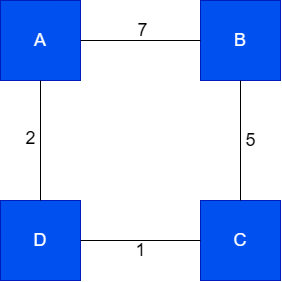
\includegraphics[width=0.3\linewidth]{DV-routing-example-2.png}
    \caption{Schema della rete dopo la modifica}
    \label{fig:enter-label}
    }
\end{figure}
\newpage \noindent L'output in console dopo la modifica è il seguente:
\begin{lstlisting}[numbers=none]
Routing table for node A:
  Destination: A, Distance: 0, Next Hop: A
  Destination: B, Distance: 7, Next Hop: B
  Destination: D, Distance: 2, Next Hop: D
  Destination: C, Distance: 3, Next Hop: D
Routing table for node B:
  Destination: B, Distance: 0, Next Hop: B
  Destination: A, Distance: 7, Next Hop: A
  Destination: C, Distance: 5, Next Hop: C
  Destination: D, Distance: 6, Next Hop: C
Routing table for node C:
  Destination: C, Distance: 0, Next Hop: C
  Destination: B, Distance: 5, Next Hop: B
  Destination: D, Distance: 1, Next Hop: D
  Destination: A, Distance: 3, Next Hop: D
Routing table for node D:
  Destination: D, Distance: 0, Next Hop: D
  Destination: C, Distance: 1, Next Hop: C
  Destination: A, Distance: 2, Next Hop: A
  Destination: B, Distance: 6, Next Hop: C
\end{lstlisting}
Come si può notare, dopo l'abbassamento del costo dell'arco tra C e D tutti i router hanno aggiornato il proprio Distance Vector per tenere traccia di rotte più brevi.

\chapter{Considerazioni finali}
Il corretto funzionamento dei due programmi è stato testato su una macchina Windows con interprete Python 3.11.8. Si è verificata la creazione di nuovi router, il collegamento tra essi, l'invio dei Distance Vector e la modifica del peso degli archi già presenti. Per semplicità non è stato implementato un meccanismo di rimozione degli archi, tuttavia con la soluzione fornita è facilmente implementabile. 
\end{document}
